% Compile with XeLaTeX. Chinese: 標楷體; Latin: Times New Roman.
\documentclass[12pt,a4paper]{article}
\usepackage[margin=16mm,top=15mm,bottom=16mm]{geometry}
\usepackage{fontspec,xeCJK}
\setmainfont{Times New Roman}
\setCJKmainfont{標楷體}[AutoFakeBold=1.4]
\setCJKsansfont{標楷體}[AutoFakeBold=1.4]
\usepackage{unicode-math}
\setmathfont{TeX Gyre Termes Math}
\usepackage{amsmath,booktabs,array,multirow,enumitem,titlesec,caption,needspace}
\usepackage{tikz}
\usetikzlibrary{arrows.meta,positioning,calc,shapes.geometric}
\usepackage[hidelinks]{hyperref}
\definecolor{navy}{HTML}{243D53}
\definecolor{blue}{HTML}{39698B}
\definecolor{orange}{HTML}{A96029}
\definecolor{green}{HTML}{287564}
\definecolor{red}{HTML}{A5413C}
\definecolor{pale}{HTML}{F3F5F6}
\hypersetup{pdftitle={Clock Buffer Insertion：合法建構與拓樸／座標混合最佳化},
  pdfauthor={李品翰 M11507401},pdfsubject={CAD Project 2 research report}}
\titleformat{\section}{\large\bfseries\color{black}}{\thesection}{0.6em}{}
\titleformat{\subsection}{\normalsize\bfseries\color{black}}{\thesubsection}{0.5em}{}
\titlespacing*{\section}{0pt}{7pt}{3pt}
\titlespacing*{\subsection}{0pt}{5pt}{2pt}
\renewcommand{\figurename}{圖}
\renewcommand{\tablename}{表}
\setlength{\parindent}{2em}
\setlength{\parskip}{2pt}
\setlength{\textfloatsep}{7pt}
\setlength{\intextsep}{6pt}
\setlength{\abovedisplayskip}{4pt}
\setlength{\belowdisplayskip}{4pt}
\captionsetup{font=normalsize,labelfont=bf,labelsep=quad,skip=3pt}
\setlist[itemize]{leftmargin=1.5em,itemsep=1pt,topsep=2pt,parsep=0pt}
\renewcommand{\arraystretch}{1.12}
\newcommand{\rDelta}{\Delta}
\newcommand{\rScore}{Q}
\newcommand{\rCost}{C}
\tikzset{edge/.style={-{Stealth[length=2mm]},line width=.65pt},
  sink/.style={circle,fill=blue,draw=blue,inner sep=2pt},
  buf/.style={rectangle,draw=navy,fill=white,minimum size=5mm,inner sep=2pt},
  length/.style={fill=white,inner sep=1pt,text=navy},
  box/.style={draw=navy,rounded corners=2pt,fill=pale,align=center,
    text width=35mm,minimum height=12mm,inner sep=3pt}}

\begin{document}
\begin{center}
  {\LARGE\bfseries Clock Buffer Insertion}\\[-1pt]
  {\large 合法建構與拓樸／座標混合最佳化}\\[3pt]
  李品翰\quad M11507401
\end{center}
\vspace{-5pt}

\section{方法概觀：建構合法樹，再改善 Score}
本方法先建構合法樹並以局部搜尋改善，作為模擬退火（SA）的初始解；
SA 再探索樹的拓樸（parent-child 關係），交由線性規劃（LP）求解此拓樸下的
buffer 座標。候選通過整數座標的合法性驗證後，
以 skew $\rDelta$ 與總 buffer 成本 $\rCost$ 計算
$\rScore=w\rDelta+\rCost$，$w$ 為輸入指定的 skew 權重。
SA 可暫時接受較差的合法解，以探索其他拓樸；另外保存歷來最佳合法解，
在時間用完時輸出。

\section{合法樹建構：空間分組、relay 與互補建構}
\subsection{空間分組與分支 buffer 放置}
先檢查 SRC 直連所有 sinks 是否合法；不可行時，比較 sinks 的 $x$、$y$
座標跨度，依跨度較大的座標排序，再按數量分成兩組，遞迴建立分支。
此分組兼顧兩組的數量平衡與空間接近程度（圖~\ref{fig:construction} 左）。
合併兩棵子樹時，在兩個 root 的中點及到達時間平衡位置採樣新分支
buffer 座標。對內部最長路徑較長的子樹，嘗試縮短新 buffer 到其 root
的連線，以縮小合併後的 skew。若直接連接超出 driver 的輸出線長總和上限，
插入單輸出 buffer（relay）拆段接續。

\begin{figure}[htbp]
\centering
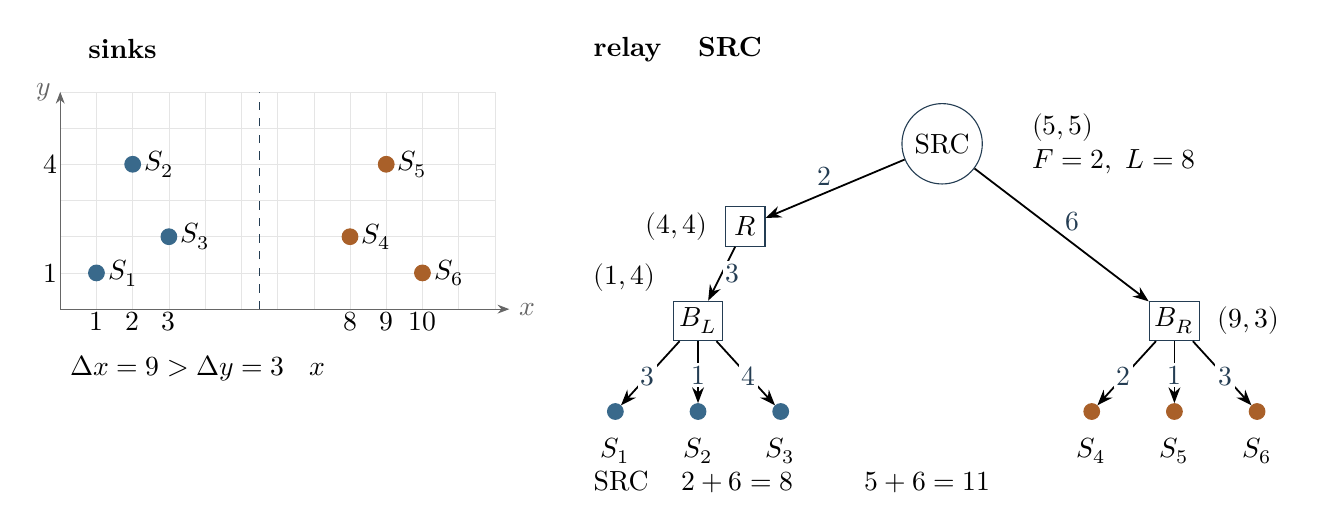
\begin{tikzpicture}[font=\normalsize]
  \node[anchor=west,text=black] at (0,4.9) {\textbf{按 sinks 座標分組}};
  \begin{scope}[shift={(0cm,1.6cm)},x=4.6mm,y=4.6mm]
    \draw[step=1,black!10,very thin] (0,0) grid (12,6);
    \draw[-{Stealth[length=1.5mm]},black!60] (0,0)--(12.4,0) node[right] {$x$};
    \draw[-{Stealth[length=1.5mm]},black!60] (0,0)--(0,6) node[left] {$y$};
    \draw[navy,dashed] (5.5,0)--(5.5,6);
    \foreach \x in {1,2,3,8,9,10}
      \node[below,inner sep=1pt] at (\x,0) {$\x$};
    \foreach \y in {1,4}
      \node[left,inner sep=1pt] at (0,\y) {$\y$};
    \foreach \x/\y/\s in {1/1/1,2/4/2,3/2/3}
      \node[sink,label={[inner sep=1pt]right:$S_{\s}$}] at (\x,\y) {};
    \foreach \x/\y/\s in {8/2/4,9/4/5,10/1/6}
      \node[sink,fill=orange,draw=orange,label={[inner sep=1pt]right:$S_{\s}$}] at (\x,\y) {};
  \end{scope}
  \node[anchor=west] at (0,0.85) {$\Delta x=9>\Delta y=3$，按 $x$ 切分};
  \node[anchor=west,text=black] at (6.65,4.9) {\textbf{relay 分攤 SRC 的輸出線長}};
  \node[draw=navy,circle,inner sep=3pt] (src) at (11.2,3.7) {SRC};
  \node[right=5mm of src,align=left] {$(5,5)$\\$F=2,\ L=8$};
  \node[buf] (r) at (8.7,2.65) {$R$};
  \node[left=1mm of r] {$(4,4)$};
  \node[buf] (bl) at (8.1,1.45) {$B_L$};
  \node[buf] (br) at (14.15,1.45) {$B_R$};
  \draw[edge] (src)--node[length,above left] {$2$}(r);
  \draw[edge] (r)--node[length,right] {$3$}(bl);
  \draw[edge] (src)--node[length,above right] {$6$}(br);
  \foreach \x/\i/\d in {7.05/1/3,8.1/2/1,9.15/3/4}{
    \node[sink] (l\i) at (\x,0.3) {};
    \node[below=1mm of l\i] {$S_{\i}$};
    \draw[edge] (bl)--node[length,pos=.55] {$\d$}(l\i);
  }
  \foreach \x/\i/\d in {13.1/4/2,14.15/5/1,15.2/6/3}{
    \node[sink,fill=orange,draw=orange] (q\i) at (\x,0.3) {};
    \node[below=1mm of q\i] {$S_{\i}$};
    \draw[edge] (br)--node[length,pos=.55] {$\d$}(q\i);
  }
  \node[above left=0mm and 1mm of bl] {$(1,4)$};
  \node[right=1mm of br] {$(9,3)$};
  \node[anchor=west] at (6.65,-0.6) {SRC 輸出：$2+6=8$；直連兩分支則為 $5+6=11$};
\end{tikzpicture}
\caption{左：按 $x$ 排序後分成各三個 sinks 的兩組。右：relay 分攤 SRC 的
輸出線長，$F$ 為 fanout 上限、$L$ 為輸出線長總和上限。邊上標示 Manhattan
distance；示意位置不按比例。插入 $R$ 使 SRC 的輸出總長從 $11$ 降為 $8$，代價是增加 buffer 成本。}
\label{fig:construction}
\end{figure}

\subsection{以多種建構適應分布與型別限制}
二元樹之外，另嘗試表~\ref{tab:construction} 的建構，以利用多輸出型別、
群聚分布或有限空位。relay 鏈的型別組合以動態規劃（DP）估計成本，
放置時再檢查邊界與座標占用。完整候選樹需通過座標唯一、連通、無環、fanout
及\textbf{各 driver 輸出線長總和}的檢查，才能進入後續改善與 Score 比較。

\begin{table}[htbp]
\centering
\begin{tabular}{@{}p{31mm}p{42mm}p{94mm}@{}}
\toprule
候選建構 & 要處理的情況 & 核心做法\\
\midrule
多輸出空間樹 & 型別可接較多 children & 一次合併多組，減少分支 buffer 數。\\
分層群組 & sinks 成群分布 & 先建群內子樹，再連接各 root，嘗試減少跨群連線。\\
混合 relay 鏈 & 長線、型別線長上限不同 & 組合不同型別，以較低成本提供所需接續線長。\\
空位受限建樹 & 可放 buffer 的點少 & 以內部空位為候選 buffer 位置，枚舉 parent-child 關係並分配 sinks。\\
\bottomrule
\end{tabular}
\caption{適應型別限制與空間分布的候選建構。}
\label{tab:construction}
\end{table}

\clearpage
\section{Score 優化：局部搜尋與 SA＋LP 的分工}
\subsection{局部搜尋：分別處理成本與到達時間差}
局部搜尋嘗試刪除／合併 buffer 以降低成本，並透過移動 buffer 座標、
交換 sinks 或子樹 root 的 parent、改接 parent 來縮小到達時間差。
對過早到達的路徑插入繞路 relay，則以增加成本換取較小 skew（圖~\ref{fig:detour}）。
刪除分支 buffer 與改接其 children 也可合成一次操作，直接評估完成改接後的結果。
每個候選重新選擇型別並驗證合法性，Score 嚴格下降才替換目前解；
改善後重試相關操作，直到沒有改善或用完嘗試預算。

\begin{figure}[htbp]
\centering
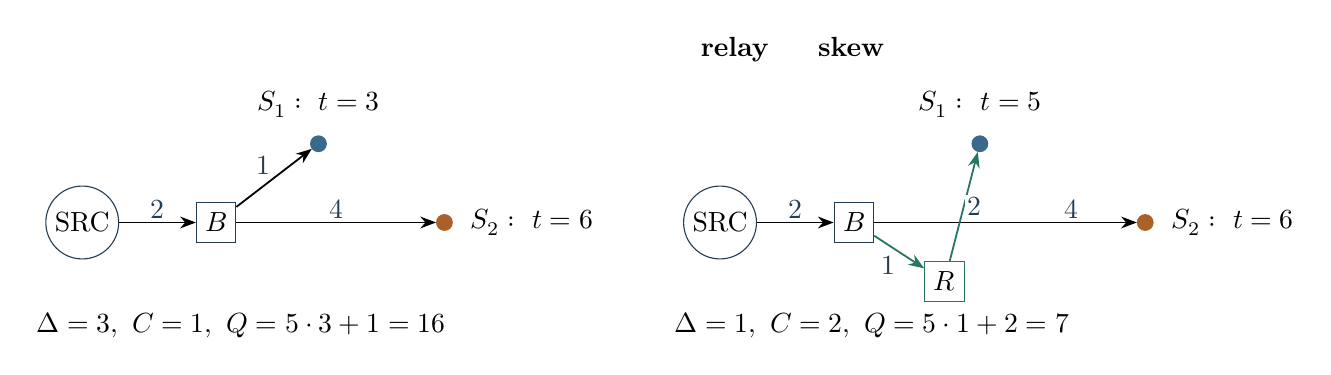
\begin{tikzpicture}[font=\normalsize]
  \node[anchor=west,text=black] at (0,2.2) {\textbf{原樹：近端過早到達}};
  \node[draw=navy,circle,inner sep=2pt] (s0) at (.7,0) {SRC};
  \node[buf] (b0) at (2.4,0) {$B$};
  \node[sink] (a0) at (3.7,1) {};
  \node[sink,fill=orange,draw=orange] (z0) at (5.3,0) {};
  \node[above=1mm of a0] {$S_1:\ t=3$};
  \node[right=1mm of z0] {$S_2:\ t=6$};
  \draw[edge] (s0)--node[length,above] {$2$}(b0);
  \draw[edge] (b0)--node[length,above left] {$1$}(a0);
  \draw[edge] (b0)--node[length,above] {$4$}(z0);
  \node[anchor=west] at (0,-1.3) {$\rDelta=3,\ \rCost=1,\ \rScore=5\cdot3+1=16$};
  \node[anchor=west,text=black] at (8.1,2.2) {\textbf{插入 relay：以成本換 skew}};
  \node[draw=navy,circle,inner sep=2pt] (s1) at (8.8,0) {SRC};
  \node[buf] (b1) at (10.5,0) {$B$};
  \node[buf,draw=green] (r1) at (11.65,-.75) {$R$};
  \node[sink] (a1) at (12.1,1) {};
  \node[sink,fill=orange,draw=orange] (z1) at (14.2,0) {};
  \node[above=1mm of a1] {$S_1:\ t=5$};
  \node[right=1mm of z1] {$S_2:\ t=6$};
  \draw[edge] (s1)--node[length,above] {$2$}(b1);
  \draw[edge] (b1)--node[length,above,pos=.75] {$4$}(z1);
  \draw[edge,green] (b1)--node[length,below left] {$1$}(r1);
  \draw[edge,green] (r1)--node[length,right] {$2$}(a1);
  \node[anchor=west] at (8.1,-1.3) {$\rDelta=1,\ \rCost=2,\ \rScore=5\cdot1+2=7$};
\end{tikzpicture}
\caption{繞路改善示例。SRC$(1,3)$、$S_1(3,4)$、$S_2(7,3)$ 與 $B(3,3)$
固定，新增 $R(3,2)$ 後，近端到達時間從 $3$ 延至 $5$。
$B$ 的輸出總長維持 $5$，$R$ 的輸出長為 $2$；兩個 buffer 成本各 $1$、
$w=5$。邊上標示 Manhattan distance，示意位置不按比例。}
\label{fig:detour}
\end{figure}

\subsection{SA 搜尋拓樸，LP 求解座標}
SA 透過更換 sink 的 parent、交換兩個 sinks 的 parent、插入／刪除 buffer，
或改接子樹 root，產生候選拓樸；也嘗試變更 buffer 型別與 child 相對 parent 的象限，
作為 LP 的驅動與位置限制。LP 固定候選拓樸及 SRC、sinks 的座標，
共同求解所有 buffer 的連續座標。固定每條邊的相對象限後，
parent-child 座標差的符號 $s_x,s_y\in\{-1,+1\}$ 隨之確定，
Manhattan distance 便可寫成線性式。
對 parent $u$ 與 child $v$，邊長 $d_{uv}$ 與從 SRC 累計的到達時間 $t$ 滿足：
\[
 d_{uv}=s_x(x_v-x_u)+s_y(y_v-y_u),\qquad t_v=t_u+d_{uv}.
\]
LP 限制 buffer 位於晶片內，且各 driver 的輸出總長符合各自上限。
以 HiGHS 的 simplex 先最小化 skew，剩餘時間足夠時，再固定此 skew
至數值誤差範圍內，最小化總線長。LP 座標取整後可能撞點或超過線長
上限，因此在附近整數格點嘗試修復。修復後依各 driver 的 fanout 與
總線長，重選最便宜的合法型別，完整驗證並計算 Score。buffer 成本
取決於各 driver 選定的型別，因此總線長用作 LP 的輔助目標。

\begin{figure}[htbp]
\centering
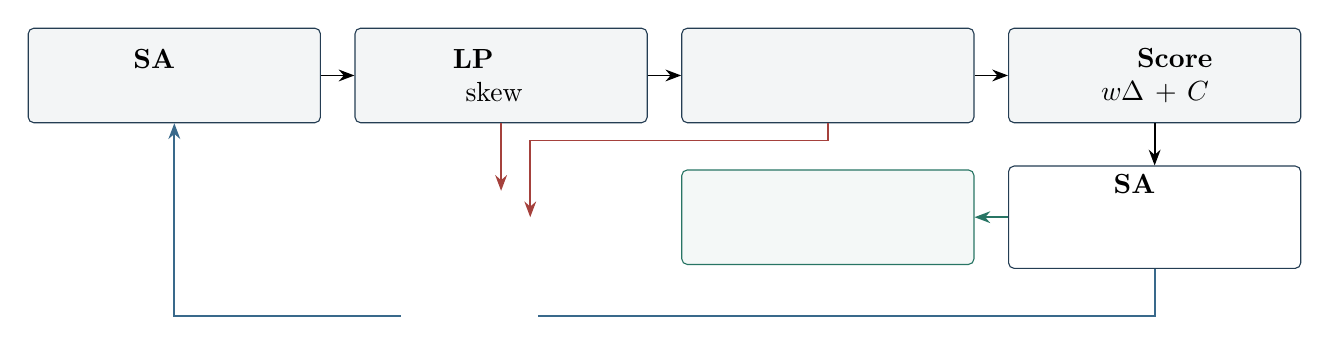
\begin{tikzpicture}[font=\normalsize]
  \node[box] (sa) at (1.8,0) {\textbf{SA 產生候選}\\拓樸／型別／象限};
  \node[box] (lp) at (5.95,0) {\textbf{LP 求解連續座標}\\先 skew，後線長};
  \node[box] (repair) at (10.1,0) {\textbf{取整、修復、驗證}\\重疊／越界／線長};
  \node[box] (score) at (14.25,0) {\textbf{計算實際 Score}\\$w\rDelta+\rCost$};
  \foreach \a/\b in {sa/lp,lp/repair,repair/score}
    \draw[edge] (\a)--(\b);
  \node[box,fill=white] (accept) at (14.25,-1.8)
    {\textbf{SA 接受判斷}\\改善／同分必收\\退步依溫度接受};
  \node[box,draw=green,fill=green!5] (best) at (10.1,-1.8)
    {\textbf{最佳合法解}\\僅收嚴格改善};
  \draw[edge] (score)--(accept);
  \draw[edge,green] (accept)--(best);
  \node[text=red,align=center] (discard) at (5.95,-1.8) {失敗／超時\\丟棄候選};
  \draw[edge,red] (lp.south)--(discard.north);
  \draw[edge,red] (repair.south)--++(0,-.22)-|(discard.east);
  \draw[edge,blue] (accept.south)--(14.25,-3.05)-|(sa.south);
  \node[fill=white,text=blue,inner sep=1pt] at (5.55,-3.05)
    {接受：更新目前解；拒絕：保留目前解};
\end{tikzpicture}
\caption{從候選拓樸、連續座標解到合法整數樹的處理流程。
LP 或整數修復失敗時保留目前解，繼續產生候選。
合法候選經接受判斷更新目前解，並在優於歷來最佳分數時更新輸出備份。}
\label{fig:search}
\end{figure}

\subsection{時間分配與降溫策略}
候選比目前解差 $\delta Q>0$ 時，以 $\exp(-\delta Q/T)$ 的機率接受。
溫度 $T$ 由早期候選的分數差校準，再逐漸降低，使後期搜尋偏重改善 Score。
產生初始解至多使用總時間的 $40\%$，提早完成則將餘下時間交給 SA。
LP 與修復受剩餘時間限制，到時輸出最佳合法解。

\clearpage
\section{實驗：各階段的改善來源與計算取捨}
以 Ubuntu 24.04、GCC 13、2 CPU／8 GiB、無網路容器執行，使用預設
CMake 建置，單次只跑一個 solver。表~\ref{tab:stages} 用目前正式版本，
每例的時間預算為 $25$ 秒，使用五個 SA seeds（1、7、17、31、101）；
依最終 Score 排序後取居中的一次，三階段均取自同次執行。
三例分別為作業範例、隨機生成例與子樹交換回歸例，均選自已知可改善的
測資，以觀察各階段的成本與 skew。隨機例的 pin 座標與 buffer library
以固定 seed 生成，包含 18 個 sinks 及兩種 buffer 型別。

\begin{table}[htbp]
\centering
\setlength{\tabcolsep}{5pt}
\begin{tabular}{@{}l r rrr rrr rr>{\bfseries}r@{}}
\toprule
 & & \multicolumn{3}{c}{首次合法解} & \multicolumn{3}{c}{SA 初始解}
 & \multicolumn{3}{c}{SA＋LP 後}\\
\cmidrule(lr){3-5}\cmidrule(lr){6-8}\cmidrule(l){9-11}
案例／sinks 數 & $w$ & $\rDelta$ & $\rCost$ & $\rScore$ & $\rDelta$ & $\rCost$ & $\rScore$
 & $\rDelta$ & $\rCost$ & $\rScore$\\
\midrule
% BEGIN STAGE ROWS -- selected same-run tuples; see data/stages.json.
作業範例（5） & 1 & 1 & 40 & 41 & 1 & 40 & 41 & 1 & 36 & 37\\
隨機生成例（18） & 1 & 1 & 119 & 120 & 20 & 44 & 64 & 19 & 40 & 59\\
子樹交換回歸例（8） & 15 & 5 & 67 & 142 & 3 & 60 & 105 & 2 & 60 & 90\\
% END STAGE ROWS
\bottomrule
\end{tabular}
\caption{同一輸入從首次合法解、建構與局部搜尋後的 SA 初始解，到 SA＋LP
結果的 skew $\rDelta$、buffer 成本 $\rCost$ 及 Score $\rScore=w\rDelta+\rCost$。
所有最終樹另以獨立整數驗證器檢查合法性。}
\label{tab:stages}
\end{table}

% BEGIN STAGE DISCUSSION -- measured same-run tuples.
作業範例的改善來自成本由 $40$ 降到 $36$。隨機生成例在建構與局部搜尋後增加 $19$
單位 skew，卻節省 $75$ 單位成本，Score 淨降 $56$；SA＋LP 再改善兩者。
子樹交換回歸例的權重 $w=15$，
最後成本同為 $60$，skew 少 $1$ 就讓 Score 再降 $15$。
五組 seeds 的最終 Score 範圍依序為 $37$、$54$--$62$、$63$--$105$；
子樹交換回歸例的變動最大，顯示該例的搜尋結果對 SA seed 敏感。
% END STAGE DISCUSSION

\subsection{消融：保留組件對合法性與 Score 的貢獻}
以同一實驗版本為完整基準，每次停用一個組件（表~\ref{tab:ablation}）。
建構與局部搜尋測 79 例；SA／LP 測 44 例，每例使用三個 seeds
（1、7、17）、至多 100 次 SA 操作，比較中位 Score。各次執行設 25 秒
上限；大樹合併另測六例，分別有 600 或 1000 個 sinks。
\begin{table}[htbp]
\centering
\begin{tabular}{@{}lrrrrr@{}}
\toprule
停用組件 & 測資數 & 較差 & 相同 & 較好 & 失敗\\
\midrule
基本局部搜尋 & 79 & 32 & 46 & 1 & 0\\
空位受限建樹 & 79 & 1 & 75 & 0 & 3\\
SA＋LP 階段 & 44 & 7 & 37 & 0 & 0\\
LP 座標求解 & 44 & 6 & 38 & 0 & 0\\
大樹 buffer 合併 & 6 & 6 & 0 & 0 & 0\\
\bottomrule
\end{tabular}
\caption{停用後相對完整基準的 Score 較差／相同／較好案例數；失敗為未產生合法輸出，另行計數。}
\label{tab:ablation}
\end{table}

空位受限建樹補足了三個密集測資的可行性。停用 LP 時沿用既有或估計
座標，仍保留整數修復與驗證；六例中位 Score 變差，支持在拓樸探索後
重新求解座標。大樹合併在六例中皆維持 skew 並降低成本；其中一個
1000-sink 案例，停用後成本 $839\to1031$，Score $1139\to1331$。
SA／LP 的 44 例僅有 1--21 個 sinks，後續需以大型測資、相同 25 秒
預算比較完整流程與停用版本，檢查求解成本增加後的收益。

\subsection{LP 目標的計算取捨}
另嘗試分別求出「只最小化 skew」與「再最小化線長」兩組座標，修復後
選 Score 較低者。八個訓練案例、五個 seeds、至多 100 次 SA 操作下，
每例中位 Score 相對預設策略的平均降幅為 $3.18\%$，同 seed 的擇優／預設
執行時間比中位數為 $1.42$。四個保留案例、五個 seeds、25 秒預算下，平均相對
Score 增加 $2.10\%$（1 勝、2 平、1 負），因此保留預設的先 skew、後線長
求解。後續可只對有潛力的候選求第二組座標，以控制每次操作的成本。

\end{document}
